% --------------------------------------------------------------
% This is all preamble stuff that you don't have to worry about.
% Head down to where it says "Start here"
% --------------------------------------------------------------
 
\documentclass[12pt]{article}

\usepackage[margin=1in]{geometry} 
\usepackage{amsmath,amsthm,amssymb}
\usepackage[margin=1in]{geometry} 
\usepackage{amsmath,amsthm,amssymb}
%\usepackage[spanish]{babel} %Castellanización
\usepackage[T1]{fontenc} %escribe lo del teclado
\usepackage{inputenc} %Reconoce algunos símbolos
\usepackage{lmodern} %optimiza algunas fuentes
\usepackage{graphicx}
\graphicspath{ {images/} }
\usepackage{hyperref} % Uso de links

% To Display Chinese words
\usepackage{xeCJK}
% To Display Code
% \usepackage{listings}
\usepackage{minted}
% To Display csv file
\usepackage{csvsimple}
\usepackage{longtable}
\usepackage{booktabs}
 
\newcommand{\N}{\mathbb{N}}
\newcommand{\Z}{\mathbb{Z}}
 
\newenvironment{theorem}[2][Theorem]{\begin{trivlist}
\item[\hskip \labelsep {\bfseries #1}\hskip \labelsep {\bfseries #2.}]}{\end{trivlist}}
\newenvironment{lemma}[2][Lemma]{\begin{trivlist}
\item[\hskip \labelsep {\bfseries #1}\hskip \labelsep {\bfseries #2.}]}{\end{trivlist}}
\newenvironment{exercise}[2][Exercise]{\begin{trivlist}
\item[\hskip \labelsep {\bfseries #1}\hskip \labelsep {\bfseries #2.}]}{\end{trivlist}}
\newenvironment{problem}[2][Problem]{\begin{trivlist}
\item[\hskip \labelsep {\bfseries #1}\hskip \labelsep {\bfseries #2.}]}{\end{trivlist}}
\newenvironment{question}[2][Question]{\begin{trivlist}
\item[\hskip \labelsep {\bfseries #1}\hskip \labelsep {\bfseries #2.}]}{\end{trivlist}}
\newenvironment{corollary}[2][Corollary]{\begin{trivlist}
\item[\hskip \labelsep {\bfseries #1}\hskip \labelsep {\bfseries #2.}]}{\end{trivlist}}

\newenvironment{solution}{\begin{proof}[Solution]}{\end{proof}}

% write csv content in latex 
\begin{filecontents*}{grade.csv}
name,givenname,matriculation,gender,grade
Maier,Hans,12345,m,1.0
Huber,Anna,23456,f,2.3
Weisbaeck,Werner,34567,m,5.0
\end{filecontents*}
 
\begin{document}
 
% --------------------------------------------------------------
%                         Start here
% --------------------------------------------------------------
 
\title{2019 Deep Learning and Practice \\ Lab 4 -- Back-Propagation Through Time (BPTT)}
\author{0756110 李東霖}

\maketitle
\section{Introduction}

In this project, I implemented a RNN model as binary addition. To calculate gradient of RNN model, I also implemented BPTT (Bcak-Propagation Through Time).

Some requirements as follows:

\begin{itemize}
\item Construct RNN and forward propagation
\item Back-Propagation Through Time
\item Only use \verb|Numpy| and pure python librarys.
\item Generate binary addition data
\item Train/Test RNN model
\end{itemize}

\section{Show accuracy of training episodes}

Accuracy is counting how many correct answers per 1000 episodes. Show 10000 training episodes in figure.

\begin{figure}[H]
\centering
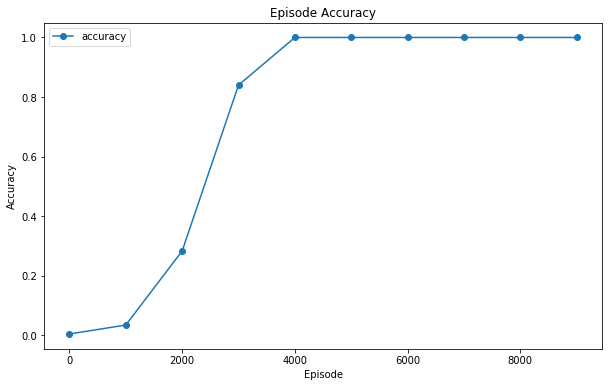
\includegraphics[width=\linewidth]{Images/PlotEpisodes.png}
\caption{Show accuracy per 1000 episodes}
\end{figure}

\section{Generate data}

I use python generator to generate binary data \verb|x, y|. To quickly convert number to binary list, I write function \verb|toBinary| to reach. The \verb|toBinary| receive number, how many digits you want convert and option for using 2's complement or not. Finally, I convert data to \verb|Variable| implemented by me and divide data into different bits. 
\par \  \par
When training model, I can get \verb|x, y| from calling \verb|next(dataset)|.

% display code
\begin{minted}[frame=lines, breaklines]{python}
def toBinaray(x, digits, complement=False):
    if complement and x < 0:
        x += (1<<(digits))
    x = abs(x)
    return [ float(int(i)) for i in list(("{:0" + str(digits) + "b}").format(x))[::-1]][:digits]

def BinaryDataset(digits=8):
    thr = (1<<(digits-1))
    while True:
        a, b = np.random.randint(0, thr, 2)
        c = a + b
        x = np.array([toBinaray(a, digits), toBinaray(b, digits)])
        y = np.array([toBinaray(c, digits)])
        yield [Variable(x.T[i:i+1, :]) for i in range(digits)], [Variable(y.T[i:i+1, :]) for i in range(digits)]

dataset = BinaryDataset(8)
x, y = next(dataset)
\end{minted}

To avoid overflow output occur in dataset, I set \verb|thr| as threshold $= 2^{d-1}$. (e.g. d$=8$, thr$=128$) Then \verb|np.random.randint| only sample integer from $[ 0, \text{thr} )$, so maximum integer is \verb|thr - 1|.

\section{Forward in RNN}

First, define our architecture, pattern and symbol for derivation.

\begin{figure}[H]
\centering
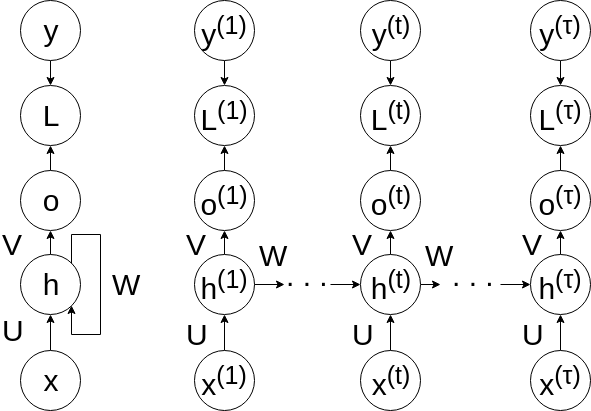
\includegraphics[width=\linewidth]{Images/RNNCG.png}
\caption{Compute Graph for my RNN}
\end{figure}

Assume have a serial data. In this lab, the serial data x is different bit of x1 and x2 and y is different bit of y.

$$ x^{(1)}, x^{(2)}, ..., x^{(\tau)} \rightarrow y^{(1)}, y^{(2)}, ..., y^{(\tau)} $$

e.g. 0b0010 + 0b1010 = 0b1001

$$
\begin{bmatrix}
0&1\\
\end{bmatrix},
\begin{bmatrix}
0&0\\
\end{bmatrix},
\begin{bmatrix}
1&1\\
\end{bmatrix},
\begin{bmatrix}
0&0\\
\end{bmatrix} \rightarrow
\begin{bmatrix}
1\\
\end{bmatrix},
\begin{bmatrix}
0\\
\end{bmatrix},
\begin{bmatrix}
0\\
\end{bmatrix},
\begin{bmatrix}
1\\
\end{bmatrix}
$$

General forward propagation : 

\begin{equation}
h^{(t)} = \sigma (a^{(t)}), \space a^{(t)} = b + Wh^{(t-1)} + Ux^{(t)}
\end{equation}

\begin{equation}
o^{(t)} = c + Vh^{(t)}
\end{equation}

\begin{equation}
\hat{y}^{(t)} = \varphi(o^{(t)})
\end{equation}

\begin{equation}
L^{(t)} = \text{loss}(\hat{y}^{(t)}, y^{(t)})
\end{equation}

RNN use previous hidden output to foward new hidden output. This is why RNN call Recurrent Neural Network. 
\par \ \par
In order to implement a RNN model, I define activation and loss function :

\begin{equation}
\sigma(x) = tanh(x)
\end{equation}

\begin{equation}
\varphi(x) = \text{softmax}(x)
\end{equation}

\begin{equation}
\text{loss}(\hat{y}, y) = \text{NLLLoss}(\hat{y}, y) = -log \prod_i (\hat{y}_i)^{y_i}
\end{equation}

But in my implement, I combine softmax and nllloss as cross entropy loss. Because the cross entropy loss more easily calculate gradient.
\par \ \par
My parameters in RNN model as follows:

\begin{itemize}
\item U :  shape (2 x hidden-unit), use for input $x^{t}$ to hidden $h^{t}$
\item W : shape (hidden-unit x hidden-unit), use for previous hidden $h^{t-1}$ to current hidden $h^{t}$
\item V : shape (hidden-unit x 2), use for hidden $h^t$ to output $o^t$
\item b : shape (1 x hidden-unit), bias for hidden layer
\item c : shape (1 x 2), bias for output layer
\end{itemize}

\section{BPTT in RNN}

To training this model, I need to calculate gradient of all parameters in model.
$$ {\triangledown_W}^L, {\triangledown_U}^L, {\triangledown_V}^L, {\triangledown_b}^L, {\triangledown_c}^L $$

First, calculate ${\triangledown_W}^L$

$$
{\triangledown_W}^L = \sum_t \sum_i (\frac{\partial L}{\partial h_i^{(t)}}) {\triangledown_W}^{h_i^{(t)}}, 
{\triangledown_W}^{h_i^{(t)}} = \frac{\partial h_i^{(t)}}{\partial a_i^{(t)}} \frac{\partial a_i^{(t)}}{\partial W} 
$$

$$
\frac{\partial h_i^{(t)}}{\partial a_i^{(t)}} = tanh'(a_i^{(t)}) = 1 - tanh^2(a_i^{(t)}) = 1 - (h_i^{(t)})^2, \space \frac{\partial a_i^{(t)}}{\partial W} = h_i^{(t-1)}
$$

$$
{\triangledown_W}^{h_i^{(t)}} = (1 - (h_i^{(t)})^2)(h_i^{(t-1)})
$$

Second, calculate $\frac{\partial L}{\partial h_i^{(t)}}$.

$$
\frac{\partial L}{\partial h_i^{(t)}} = (\frac{\partial h_i^{(t+1)}}{\partial h_i^{(t)}} \frac{\partial L}{\partial h_i^{(t+1)}}) + (\frac{\partial o_i^{(t)}}{\partial h_i^{(t)}} \frac{\partial L}{\partial o_i^{(t)}})
$$

$$
\frac{\partial h_i^{(t+1)}}{\partial h_i^{(t)}} = \frac{\partial a_i^{(t+1)}}{\partial h_i^{(t)}} \frac{\partial h_i^{(t+1)}}{\partial a_i^{(t+1)}} = W (1 - (h_i^{(t+1)})^2)
$$

$$
\frac{\partial o_i^{(t)}}{\partial h_i^{(t)}} = V
$$

Third, calculate $\frac{\partial L}{\partial o_i^{(t)}}$

$$
\frac{\partial L}{\partial o_i^{(t)}} = \frac{\partial \hat{y}^{(t)}}{\partial o_i^{(t)}}\frac{\partial L}{\partial \hat{y}^{(t)}} = \text{softmax}'(o^{(t)}) (\frac{\partial - \sum_j y_j^{(t)}log (\hat{y}_j^{(t)})}{\partial \hat{y}^{(t)}})
$$

$$
text{softmax}'(x) = \left\{\begin{array}{ll} \text{softmax}(x_i) (1 - \text{softmax}(x_i)), \text{if i==j} \\ -\text{softmax}(x_i)\text{softmax}(x_j), \text{if i != j}\end{array}\right.
$$

$$
= \hat{y}_i^{(t)}(1 -\hat{y}_i^{(t)}) (-\frac{y_i^{(t)}}{\hat{y}_i^{(t)}}) + \sum_{j\neq i} -\hat{y}_i^{(t)}\hat{y}_j^{(t)} (-\frac{y_j^{(t)}}{\hat{y}_j^{(t)}})
$$

$$
= (\hat{y}_i^{(t)} - 1) y_i^{(t)} + \sum_{j\neq i} \hat{y}_i^{(t)}y_j^{(t)}
= ( \sum_j y_j^{(t)} ) \hat{y_i}^{(t)} - y_i^{(t)}
$$

if $\sum y{(t)}$ is one, equation can rewrite to:
\begin{equation}\label{grad:crossentropy}
\frac{\partial L}{\partial o_i^{(t)}} = \hat{y_i^{(t)}} - y_i^{(t)}   
\end{equation}

And need final time layer hidden gradient to start BPTT.

\begin{equation}
{\triangledown_{h_i^{(\tau)}}}^L = \frac{\partial o_i^{(\tau)}}{\partial h_i^{(\tau)}} \frac{\partial L}{\partial o_i^{(\tau)}} = V(\hat{y_i^{(\tau)}} - y_i^{(\tau)})
\end{equation}

Finally, get all equations for computing gradient : 

\begin{equation}
\frac{\partial L}{\partial h_i^{(t)}} = W(1 - (h_i^{t+1})^2) \frac{\partial L}{\partial h_i^{(t+1)}} + V(\hat{y_i^{(t)}} - y_i^{(t)})    
\end{equation}

\begin{equation}
{\triangledown_W}^L = \sum_t \sum_i (\frac{\partial L}{\partial h_i^{(t)}}) (\frac{\partial h_i^{(t)}}{\partial W}) = \sum_t \sum_i \frac{\partial L}{\partial h_i^{(t)}} (1 - (h_i^{(t)})^2)(h_i^{(t-1)})
\end{equation}

\begin{equation}
{\triangledown_U}^L = \sum_t \sum_i (\frac{\partial L}{\partial h_i^{(t)}}) (\frac{\partial h_i^{(t)}}{\partial U}) = \sum_t \sum_i \frac{\partial L}{\partial h_i^{(t)}} (1 - (h_i^{(t)})^2)(x_i^{(t)})
\end{equation}

\begin{equation}
{\triangledown_V}^L =  \sum_t \sum_i (\frac{\partial L}{\partial o_i^{(t)}}) (\frac{\partial o_i^{(t)}}{\partial V}) = \sum_t \sum_i (\hat{y_i^{(t)}} - y_i^{(t)}) h_i^{(t)} 
\end{equation}

\begin{equation}
{\triangledown_b}^L = \sum_t \sum_i (\frac{\partial L}{\partial h_i^{(t)}}) (\frac{\partial h_i^{(t)}}{\partial b}) = \sum_t \sum_i \frac{\partial L}{\partial h_i^{(t)}} (1 - (h_i^{(t)})^2)    
\end{equation}

\begin{equation}
{\triangledown_c}^L = \sum_t \sum_i (\frac{\partial L}{\partial o_i^{(t)}}) (\frac{\partial o_i^{(t)}}{\partial c}) = \sum_t \sum_i \hat{y_i^{(t)}} - y_i^{(t)} 
\end{equation}

\section{Code explanation}

I can directly declare $U, W, V, b, c$ parameters and write equation to calculate gradient. But I also want to understand pytorch \verb|autograd|. Because of that, I implement a data node class called \verb|Variable| to store compute graph and calculate gradient through graph.

\subsection{Calculating Compute Graph Gradient}

To store compute graph, I store what variable and operation that create this variable in \verb|fn|. And I want to trace how many variable be created by this variable, I store them into \verb|child|. The \verb|ready| bool means this variable already finish computing gradient from target to it self. \verb|data| stores variable content as \verb|ndarray|. \verb|grad| stores variable gradient as \verb|ndarray|.

\begin{minted}[frame=lines, breaklines]{python}
class Variable():
    def __init__(self, data, T=None, grad=None, copy=True):
        if data is None or type(data) != np.ndarray:
            raise AttributeError('Wrong data type')
        
        if copy:
            self.data = data.copy()
        else:
            self.data = data
        if grad is None:
            grad = np.zeros_like(self.data)
        self.grad = grad
        if T is None:
            T = Variable(self.data.T, self, self.grad.T, copy=False)
        self.T = T
        self.fn = None
        self.child = []
        self.ready = False
    
    def zero_grad(self):
        self.grad[:,:] = 0.0
        self.child = []
        self.ready = False
\end{minted}

To easily use this class, I overloaded the operator about it. When this class do operation with the same other, That overload method will record some info about compute graph. The operator overloaded as follows:

\begin{itemize}
\item add (matrix element-wise addition)
\item sub (matrix element-wise subtraction)
\item mul (matrix element-wise multiple)
\item matmul (matrix multiple)
\end{itemize}

I just put one of them as example to explain my code. Other overload methods are similar but calculating gradient are different. 

\begin{minted}[frame=lines, breaklines]{python}
class Variable():
    # Omit sth ...
    def __matmul__(self, b):
        c = Variable(np.matmul(self.data, b.data))
        c.fn = [Variable.__grad_matmul__, self, b]
           
        self.child.append(c)
        b.child.append(c)
        return c
    
    def __grad_matmul__(self, a, b):
        a.grad += np.matmul(self.grad, b.data.T)
        b.grad += np.matmul(a.data.T, self.grad)
\end{minted}

Assume \verb|A|, \verb|B| is Variable class. When do matrix multiple (\verb|C = A @ B|), python will send \verb|A| as \verb|self| and \verb|B| as \verb|b| into \verb|__matmul__| method. So I can store any compute graph.
\par \ \par

I also need some special operation in RNN model.

\begin{itemize}
\item tanh    
\item crossentropy
\end{itemize}

\begin{minted}[frame=lines, breaklines]{python}
class Variable():
    # Omit sth ...
    def crossentropy(self, target):
        s = self.softmax(1)
        if type(target) is Variable:
            target = target.data
            
        target = target.astype(np.int)
        
        if target.shape[0] > 1:
            slis = tuple(zip(range(target.shape[0]), target))
        else:
            slis = (0, target[0])
        
        c = Variable(np.array(np.sum(-np.log(s[slis]))))
        c.fn = [Variable.__grad_corssentropy, self, target]
        
        self.child.append(c)
        return c
    
    def __grad_corssentropy(self, a, target):
        y = np.zeros_like(a.grad)
        if target.shape[0] > 1:
            slis = tuple(zip(range(target.shape[0]), target))
        else:
            slis = (0, target[0])
            
        y[slis] = 1.0
        a.grad += (a.softmax(1) - y)
\end{minted}

I combine softmax and nllloss as one operation. It help me easily compute gradient. (like \ref{grad:crossentropy})
\par \ \par

If finish forward propagation, whole compute graph have been store in multi Varaible class. I can call \verb|backward| method on loss Variable then it will do BPTT through compute graph.

\begin{minted}[frame=lines, breaklines]{python}
class Variable():
    # Omit sth ...
    def backward(self, backward_grad):
        if type(backward_grad) is Variable:
            backward_grad = backward_grad.data
        
        if backward_grad.shape != self.data.shape:
            raise AttributeError('Wrong backward grad shape {} != {}'.format(backward_grad.shape, self.data.shape))
        
        self.grad = backward_grad
        self.__backward()
    
    def __backward(self):
        if self.fn is None:
            return;
        
        # check self grad is ready, trace child variables
        self.ready = True
        for child in self.child:
            self.ready &= child.ready
        
        if not self.ready:
            return;
        
        backward_op = self.fn[0]
        
        backward_op(self, *self.fn[1:])
        
        for v in self.fn[1:]:
            if type(v) is Variable:
                v.__backward()
\end{minted}

To start backward, I need backward gradient from target (e.g. Loss result $L$) to this Variable. Then check \verb|fn| find compute graph. Second, check \verb|child| ready to sure self gradient has been calculated. Third, call backward operation paired with forward operation (e.g. \verb|__add__| mapping \verb|__grad_add__|) to calculate gradient of previous creator. If recursive loop finish, that means already calculated all gradient of compute graph.

\subsection{Build RNN}

Now, I can easily build model by RNN forward equation.

\begin{minted}[frame=lines, breaklines]{python}
class RNN():
    def __init__(self, in_channels, out_channels, hidden_channels):
        self.U = Variable(np.random.uniform(-1,1, (in_channels, hidden_channels)))
        self.W = Variable(np.random.uniform(-1,1, (hidden_channels, hidden_channels)))
        self.V = Variable(np.random.uniform(-1,1, (hidden_channels, out_channels)))
        self.b = Variable(np.random.uniform(-1,1, (1, hidden_channels)))
        self.c = Variable(np.random.uniform(-1,1, (1, out_channels)))
    
    def forward(self, x):
        t = len(x)
        self.h = None
        y = []
        
        for i in range(t):
            a = self.b + (x[i] @ self.U)
            if self.h is not None:
                a += (self.h @ self.W)
        
            self.h = a.tanh()
            
            o = self.c + (self.h @ self.V)
            y.append(o)
        
        return y
    
    def zero_grad(self):
        self.U.zero_grad()
        self.W.zero_grad()
        self.V.zero_grad()
        self.b.zero_grad()
        self.c.zero_grad()
    
    def step(self, lr=1e-1):
        self.U.data -= lr * self.U.grad
        self.W.data -= lr * self.W.grad
        self.V.data -= lr * self.V.grad
        self.b.data -= lr * self.b.grad
        self.c.data -= lr * self.c.grad
\end{minted}

I assume shape of input \verb|x| is (T, D). T means how many bit in this serial data. (In this lab, it is 8) D means how many number in this bit. (In this lab, it is 2) Then I use forward equation to generate output. The noteworthy thing is the initial hidden unit $h$ is None or zero matrix. Because the random initial will let model output is unstable, I don't want to it. \verb|zero_grad| is for cleaning gradient buffer. \verb|step| is for updating parameters.

\subsection{Calculate Loss and Update}

\begin{minted}[frame=lines, breaklines]{python}
x, y = next(dataset)
    
model.zero_grad()
    
output = model.forward(x)
    
loss = [output[i].crossentropy(y[i]) for i in range(len(y))]
    
for l in loss[::-1]:
    l.backward(np.array(1))
        
model.step(1e-2)
\end{minted}

First, I clear gradient buffer to prevent previous buffer value. Second, because my RNN model is multiple output in one input data, I need to calculate loss each value in output. Then I call method \verb|backward| from back to front by each loss. After the for loop, I will get gradient in each \verb|grad| variable. Therefore I can call \verb|step| with learning rate to update parameters of model.

\newpage

\section{Discussion}

\subsection{Extend number of binary bit when evaluation}

I think this model can store the carry information into hidden output. And the hidden output can influence the model output. Therefore the model should be trained by 8 bits but it can handle more than 8 bits. I do experiment to prove it.

\begin{figure}[H]
\centering
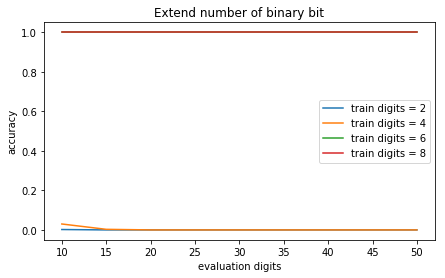
\includegraphics[width=\linewidth]{Images/ExtendED.png}
\caption{Extend number of digits when evaluation}
\end{figure}

Very interesting ! I found model by training with little digits can handle more digits. This result means the hidden unit of model can represent the carry information to next point in time series.

\subsection{How many hidden unit do task need}

I consider this binary addition task is simple so the model should be decreased number of hidden unit. I do experiment to find how many hidden unit need.

\begin{figure}[H]
\centering
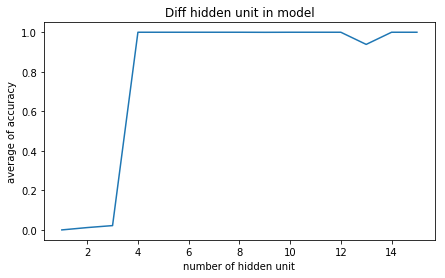
\includegraphics[width=\linewidth]{Images/DiffHU.png}
\caption{Different Hidden unit in model}
\end{figure}

The figure shows the minimum number of hidden unit is 4.

% display csv content
% \csvautotabular{path/to/csv.csv}

% display content in latex
%\ \par
%This table
%\par
%\csvautotabular{grade.csv}
%\par \ \par

%This book table with caption
%\par
%\begin{table}[H]
%    \centering
%    \csvautobooktabular{grade.csv}
%    \caption{Hi i am caption}
%    \label{tab:my_label}
%\end{table}


% --------------------------------------------------------------
%     You don't have to mess with anything below this line.
% --------------------------------------------------------------
 
\end{document}